Differences in gender are well-known features of economic and social life. This paper investigates how participation in enriched early childhood programs differently enhances the lives of disadvantaged boys and girls, and whether they enhance or reduce gender gaps among disadvantaged children.

There is a rich literature in psychology on the greater vulnerability of boys to adverse life conditions. As a group, girls mature earlier, are more resilient to adversity, and perform better on a variety of lifetime outcomes.\footnote{See \cite{Schore_2017_IMHJ} for an extensive survey. Economists have contributed to this literature. See, e.g., \cite{Autor-etal_2015_Family-Disadvantage}.} Less is known about effective strategies for reducing the vulnerability of boys to disadvantage. This paper investigates this questions using data from a randomized controlled trial of a prototypical intensive early childhood program that enriched the early lives of disadvantaged children. The program is a template for many current and proposed early interventions. It starts at eight weeks of age and continues through age 5. Participants and controls are followed through age 34 with data collected at all stages of the life cycle.

There are positive life-cycle impacts of the program for both genders. However, there are substantial differences in impact by gender that vary by the domain studied. The program studied differentially promotes the earnings, employment and health of males and reduces their participation in crime. It differentially enhances the IQ, cognition and education of girls. We investigate the sources of these differences. Home care versus low quality center care on children by gender. Boys placed in low quality center environments do much worse than girls. This is consistent with a large body of work in psychology on vulnerability and the importance of early attachment on the lives of boys. Boys benefit relatively more from high quality center care than girls, although both genders benefit.

We analyze data from the Carolina Abecedarian Project (ABC) and its sister program, Carolina Approach to Responsive Education (CARE). These programs were conducted in Chapel Hill, North Carolina for a sample of children born between 1972 and 1980. We refer to the combined programs as ABC/CARE.

To preview of our analysis, we report gender differences of outcomes in Figure~\ref{fig:proportion}. \textbf{[JJH: Why these 3 outcomes? We need categories.][We edited the figures and the description.]} We report the proportion of outcomes, by outcome category, for which the males outperform the females. We do this for the control group and the treatment group separately to establish a baseline gender difference and the value-added of treatment. Baseline, males have higher IQ scores, employment, parental income, and crime. They also do better when considering across all outcome categories. Treatment drastically narrows the gap between males and females for achievement, with all achievement measures favoring females in the treatment group. Education is another outcome category for which treatment narrows the gender gap. Males have (non-significantly) higher educational attainment in the control group with over 50\% of the education outcomes favoring males. In the treatment group, however, less than 25\% of the education outcomes favor males. This pattern also appears for employment outcomes and grouping across all outcome categories. 

\textbf{[JJH: Too narrowly focused -- why pick these 3? Need effect by category.]}
\textbf{[JJH: Why these measures?][We have changed these plots to show (a) the control-group gender differences and (b) the value added of treatment. We thought these measures were illustrative and showed interesting results.] [JJH: Figures way too busy. Crime, health, earnings, cognition, education.]} \\
\textbf{[We changed the plots to show the proportion of outcomes, by category, for which the males outperform the females.]}

\begin{figure}[!htbp]
\centering
\caption{Proportion of Outcomes Males $>$ Females, by Outcome Category}
\label{fig:proportion}
\begin{subfigure}[h]{0.8\textwidth}
	\centering
	\caption{Control Gender Gaps}
	\label{fig:means-sociab}
	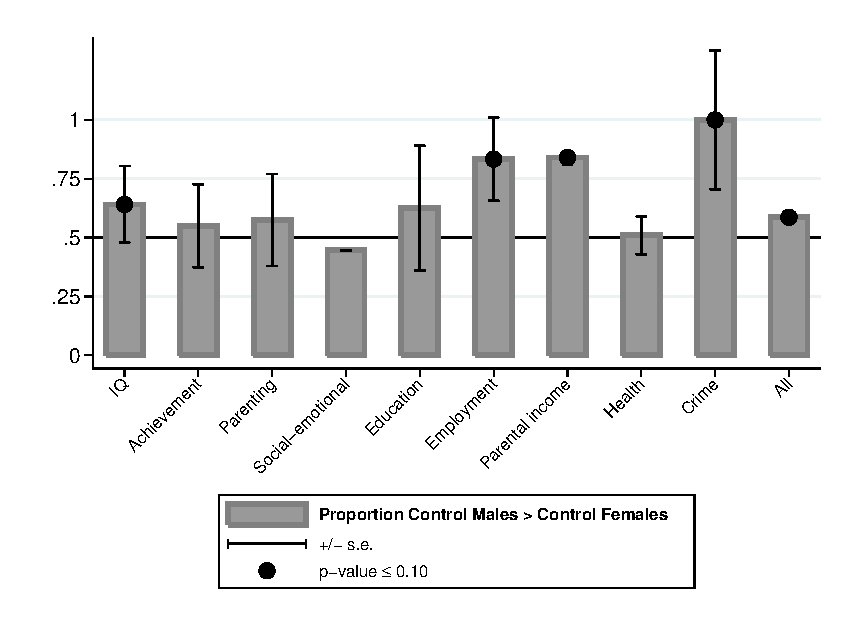
\includegraphics[width=\textwidth]{output/gendergaps-fullcontrol}
\end{subfigure}

\begin{subfigure}[h]{0.8\textwidth}
	\centering
	\caption{Treatment Gender Gaps}
	\label{fig:means-years}
	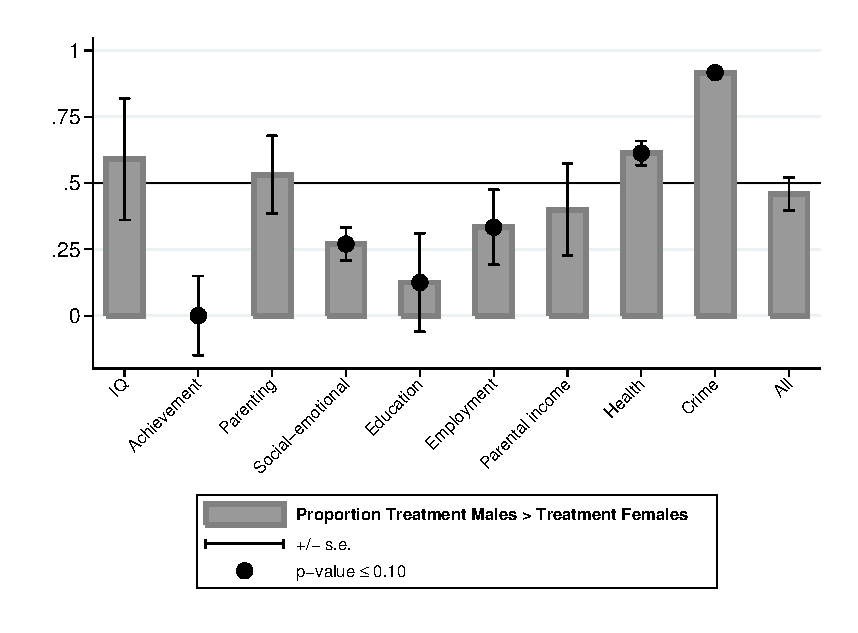
\includegraphics[width=\textwidth]{output/gendergaps-treatment}
\end{subfigure} 
\footnotesize \justify
Note: These plots show the proportion of outcomes, by outcome category, for which the males' mean is larger than the females' mean. The standard errors and the $p$-values are computed using 100 bootstraps. The $p$-values are one-sided and test the null hypothesis that the proportion of outcomes is greater than $\frac{1}{2}$ The crime outcomes are all coded so that a higher value indicates more criminal activity. All other outcome categories have higher values corresponding to socially desirable outcomes. 
\end{figure}

Table~\ref{tab:proportion-table} summarizes the gender gaps in these plots as well as those when considering the alternative setting of the control-group children. In the full control group, the proportions of outcomes for which males do better than females is higher than $\frac{1}{2}$ for a majority of the outcome categories. The exceptions are social-emotional skills, in which females surpass males, and crime, in which the outcomes are coded such that higher values correspond with more criminal activity. Treatment reverses the gaps for achievement, education, employment, parental income, and all the outcomes taken together. It only widens the gap for health, with treatment causing males to achieve better health outcomes. When considering the control-group subjects who stay at home, females have better health outcomes and commit more crimes. Both of these are reduced with treatment. Finally, the males who attend alternative preschool do not outperform females on any of the outcome categories that predominantly include early outcomes. This indicates an early-life disadvantage that treatment partially corrects.

\begin{table}[H]
\centering
\caption{Summary of Proportion of Outcomes Males $>$ Females}
\label{tab:proportion-table}
\begin{threeparttable}
\begin{tabular}{l | c |c |c| c}
\toprule
& (1) & (2) & (3) & (4) \\
Category & Control Group  &  Control Group &  Control Group &  Treatment \\
	&				&	Stay at Home		& Alternative Preschool &  Group \\
\midrule  
IQ 								& \checkmark &  \checkmark* & $\times$&\checkmark \\
Achievement						& \checkmark &  \checkmark* &$\times$ & $\times$* \\
Parenting							& \checkmark&  \checkmark* &$\times$ & \checkmark \\
Social-emotional					& $\times$&$=$ &$\times$* &$\times$* \\
Education							& \checkmark&\checkmark & $=$ &$\times$* \\
Employment						&  \checkmark* &  \checkmark* &  \checkmark* &$\times$* \\
Parental income					&  \checkmark* &\checkmark & \checkmark & $\times$\\
Health 							& \checkmark &$\times$ &\checkmark &  \checkmark* \\
Crime							&  \checkmark* &  $=$ & \checkmark* &  \checkmark* \\
\midrule
All								&  \checkmark* &\checkmark*&  $\times$ & $\times$\\
\bottomrule
\end{tabular}
\begin{tablenotes}
\footnotesize
\item Note: This table summarizes comparison of gender gaps across outcome categories by different groups. A checkmark indicates that the proportion of outcomes in the corresponding category is larger than $\frac{1}{2}$, meaning that males outperform females. A checkmark with an asterisk indicates that the proportion is significantly larger than $\frac{1}{2}$. Column (1) is the difference between males and females in the full control group.  Column (2) is the difference between males and females in the control group only considering those who stayed at home. Column (3) is the difference between males and females in the control group only considering those who attended alternative preschools. Column (4) is the difference between males and females in the treatment group.
\end{tablenotes}
\end{threeparttable}
\end{table}

Many studies have shown the potential for early-life interventions to improve the skills of children, especially those from disadvantaged families.\footnote{\citet{Currie_2011_AER,Elango_Hojman_etal_2016_Early-Edu}.} Several of these studies separate analysis by gender and find that males and females benefit differently from early childhood education. For example, \citet{Heckman_Moon_etal_2010_QE} and \citet{Garcia_Heckman_Leaf_etal_2017_Comp_CBA_Unpublished}, analyze randomized controllled trials with long-term data follow-ups, find that intervening early in life more positively affects education for females and labor market and health outcomes for males. Other studies analyzing programs with shorter-term data also find gender differences in early skills and academic outcomes.\footnote{\citet{Deming_2009_AEJAE,Ou_Reynolds_2010_Mechanisms_CYSR,Magnuson_Kelchen_Duncan_etal_2016_ECRQ}.} None of these studies have examined the gender gap and how treatment alters it.

This paper studies the treatment effects of ABC/CARE by gender. We report standard treatment effects comparing the treatment and control groups. This considers the treatment effect given that the control-group families select the ``next best'' early childhood option for their children. \textbf{[JJH: No, we also study by alt.]} This option can include staying at home or attending other center-based care that was of lower quality than the ABC/CARE program.\footnote{Historical documentation, records, and evidence from knowledgeable individuals indicate that although these alternate centers followed state and federal standards, they were of lower quality than the ABC/CARE program.} \textbf{[JJH: High quality vs low quality center. High quality vs home.][We expanded this paragraph to make the comparisons and their purpose more explicit.]} Unlike previous studies analyzing ABC/CARE, we additionally compute treatment effects comparing the treatment group to the control group fixing those in the control group to these two alternate counterfactuals.\footnote{Previous studies presenting treatment effects of ABC and CARE include \citet{Ramey_etal_1985_Project-CARE_TiECSE, Clarke_Campbell_1998_ABC_Comparison_ECRQ,Campbell_Pungello_etal_2001_DP,Campbell_Ramey_etal_2002_ADS,Campbell_Wasik_etal_2008_ECRQ,Campbell_Conti_etal_2014_EarlyChildhoodInvestments}.}$^,$\footnote{See \cite{Heckman_1992_randomization}, \cite{Heckman_Hohmann_etal_2000_QJE}, and \cite{Kline_Walters_2016_QJE} for work related to control substitution.} This allows us to speak to two policy-relevant comparisons: the treatment effect of ABC/CARE relative to staying at home and the effect of ABC/CARE relative to low-quality alternative preschool. 

We consider a total of 95 outcomes that we classify in Appendix~\ref{appendix:results}. \textbf{[JJH: These should go in text.][This sentence was moved from the footnote to the main text.] [JJH: We need to summarize these.][We added a summary.]} Frequent measures of cognitive, social-emotional, and parenting skills were collected during the intervention and while the subjects were in school. The researchers collected information on the subjects' academics including grade retention and special education. The adult surveys (at ages 21 and 30) cover items related to employment, post-secondary education, health, criminal activity, and family structure. When the subjects were in their mid 30s, the researchers collected administrative crime data and data from a full medical survey.

Given the large number of available variables from the numerous follow-ups, summarizing \textbf{[JJH: Effects by category.][We added plots showing the combining functions by gender in Section 6. We summarize them in the next paragraph.]} all treatment effects can overwhelm the reader. In a companion paper, \citet{Garcia_Heckman_Leaf_etal_2017_Comp_CBA_Unpublished} aggregate the treatment effects by conducting a cost/benefit analysis. They show that the benefits from ABC/CARE are largely driven by its effects on males. The benefit/cost ratio is 10.19 for males and 2.61 for females. In this paper, we report treatment effects by category and the proportion of statistically significant effects. We use combining functions, which count the number of positive (and significant) treatment effects by gender. They indicate that females benefit more from the program than do males.

We find strong effects on education and employment for females with high school graduation increasing between 13 and 25 percent and employment increasing between 8 and 13 percentage points.\footnote{The range arrises from the different estimates.} Although the treatment did not increase education for males as strongly as for females, it increased employment between 11 to 19 percentage points and labor income between 19 and 24 thousand of 2014 US dollars.\footnote{Income, employment, and education were measured when the subjects were 30 years.}  For females in comparison to alternative preschool, 40\% of the education outcomes and 20\% of the employment outcomes are positive and significant. These increase to 80\% and 100\% when comparing to staying at home. The treatment advantage for males is only seen when compared to those males who attended alternative preschool, with none of the education or employment outcomes being significant and positive when compared to staying at home. \textbf{[JJH: List by category.][We added a summary of the combining functions for the relevant categories. The plots by category are now in Section 6.]}

We broaden the discussion of results to the full set of outcomes by presenting the estimates of the counts of positive treatment effects. To perform inference on these estimates, we test the hypothesis of whether the proportions are equal to 50\%. As Figure~\ref{fig:intro-cfunctions} shows, although the proportions for both genders are significantly greater than 50\%, the proportion is higher for females. When considering the proportion of outcomes that are both positive and significant at the 10\% level, we test the hypothesis whether the proportions are equal to 10\%.\footnote{Our inference accounts for the dependence across outcomes, as we explain in Section~\ref{sec:combining-functions}.} A similar pattern holds for this test as well, although the proportions are smaller. Across outcomes, the effects are stronger for males fixing the control group to alternate preschool, but stronger for females when fixing the control group to staying at home. This pattern holds in the individual treatment effects, the combining functions, and the results from \citet{Garcia_Heckman_Leaf_etal_2017_Comp_CBA_Unpublished}.

\begin{figure}[!htbp]
\centering
\caption{Proportion of Outcomes that are Positively Impacted}
\label{fig:intro-cfunctions}
	\begin{subfigure}[h]{0.7\textwidth}
	\centering
	\caption{Treatment vs. Next Best} \label{fig:ppositive10}
		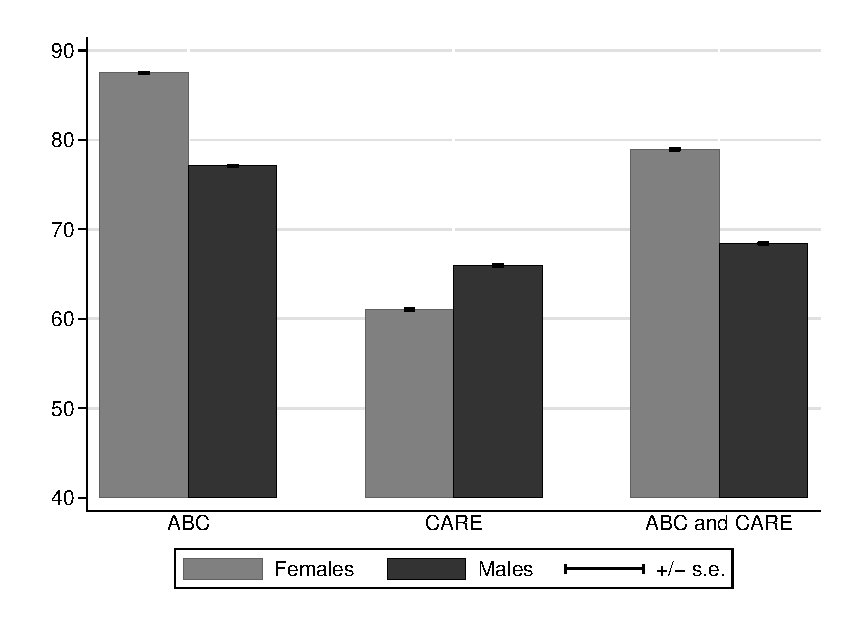
\includegraphics[width=\textwidth]{output/itt_noctrl_all.eps}
\end{subfigure}
	\begin{subfigure}[h]{0.7\textwidth}
	\centering
	\caption{Treatment vs. Next Best, Significant at 10\% Level} \label{fig:ppositive10}
		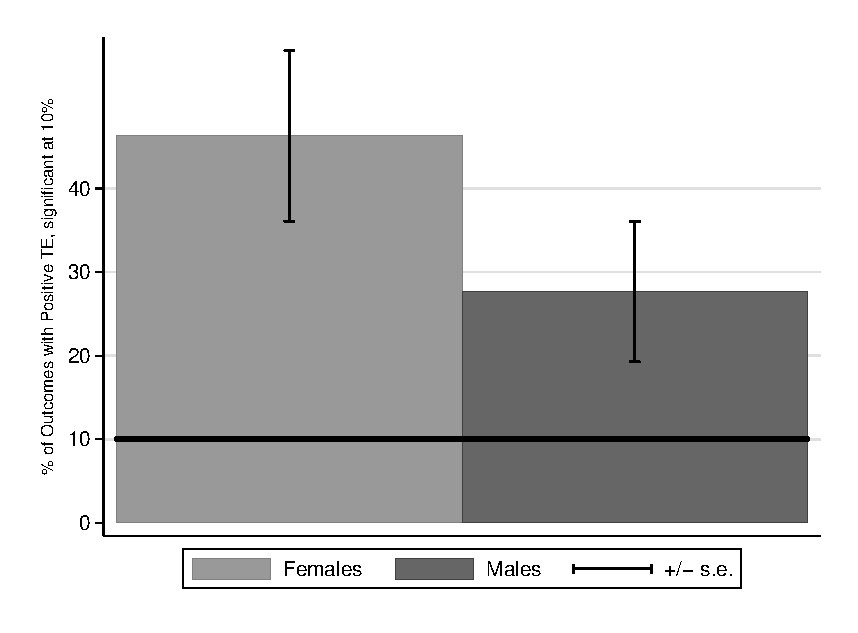
\includegraphics[width=\textwidth]{output/itt_noctrl_all_sig10.eps}
\end{subfigure}
\footnotesize \justify
Note: Panel (a) percentage of outcomes displaying a positive treatment effect, comparing treatment to next best. Panel (b) percentage of outcomes displaying a positive and statistically significant treatment effect (10\% significance level).
\end{figure}

\textbf{[JJH: Comes too early -- summarize and report later.][We added summary of the analysis in response to comments 7a and 7b to come before a summary of the treatment effects.]}

This difference in the results depending on the counterfactual, as well as the gender differences in the treatment effects, drives our discussion of the interaction between the treatment, the family inputs, and any potential alternate center-based care. The explanation that males are more fragile than females early in life is consistent with the early differences favoring females.\footnote{\citet{Kottelenberg-Lehrer_2014_Gender-Effects,Baker_Gruber_Milligan_2015_Noncog_Defects, Schore_2017_IMHJ}.} Building on this, we explore how these early-life differences evolve for specific outcomes that are central to the analysis of  \citet{Garcia_Heckman_Leaf_etal_2017_Comp_CBA_Unpublished}, such as crime and income. We find that the treatment narrows or reverses the male-female gap for many outcomes, including education and employment. Treatment widens the male-female gap for health.

The paper proceeds as follows. We describe ABC/CARE in more detail in Section~\ref{sec:data}. We then discuss the parameters of interest in Section~\ref{sec:parameters} and describe our method for summarizing over the multitude of variables in Section~\ref{sec:combining-functions}. Section~\ref{sec:treatment-effects} displays the estimates of the parameters of interest and the combining functions. We discuss suggestive mechanisms through which the early-life skill differences mediate later-life gender differences in Section~\ref{sec:gender-differences}. Section~\ref{sec:conclusion} concludes.


\textbf{[JJH: We need to report}
\begin{enumerate}[7(a)]
\item \textbf{Value added compared to home by gender (do we have results moderated by family background and by presence/absence of father?)}
\item \textbf{Comparison of control children---are girls doing better or worse?/also report moderators]}
\end{enumerate}

\textbf{[We have included plots and discussion getting at these points and will update them further by tomorrow.]}

\textbf{[JJH: Previous research on gender differences.][We are working on this and will start updating the writeup tomorrow 4/29.]}

%ee \citet{Beeghly-etal_2017_IMHJ,Dayton_2017_IMHJ,Iruka_2017_IMHJ,Schore_2017_IMHJ} for recent findings on the topic of different development of males and females early in life. 